\documentclass[12pt]{article}
\usepackage{amsfonts}
\usepackage{graphicx}
\usepackage[top=1.2in,bottom=1.2in,left=1in,right=1in]{geometry}
\title{Lecture-5 }
\begin{document}
\maketitle
\section{Neyman-Pearson Hypothesis Testing for binary channel} 
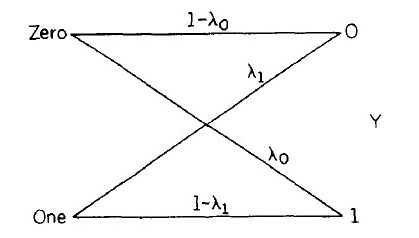
\includegraphics[scale=0.8]{img1.jpg} \\
\textbf{figure-1} The Binary Channel\\
Likelihood ratio is given by  $ L(y) = \frac{\mathbb{P}_1(y)}{\mathbb{P}_0(y)} $ \\
Decision rule for Neyman Pearson testing is given by \\

$\tilde{\delta}_{NP} (y) =\left\{ \begin{tabular}{c c c}
$1$  & $ L(y) > \eta_0$ \\ 
$\gamma_0$  & $L(y)= \eta_0$  \\
$0$  & $L(y) < \eta_0$   \\
\end{tabular}\right.$ \\

where $\eta_0$ is desired threshold for $\alpha$ level Neyman Pearson testing \\
\begin{large}

$L(0) = \frac{\mathbb{P}_1(0)}{\mathbb{P}_0(0)} = \frac{\lambda_1}{1-\lambda_0}$ ; \\


$ L(1) = \frac{\mathbb{P}_1(1)}{\mathbb{P}_0(1)} = \frac{1-\lambda_1}{\lambda_0}$;

$ L(y) = \left\{ \begin{tabular}{c c}
$\frac{\lambda_1}{1-\lambda_0}$ & $y=0$  \\ 
\\

$\frac{1-\lambda_1}{\lambda_0}$ & $y=1$
\end{tabular}\right.$
\end{large}  \\


Assume $\lambda_0 + \lambda_1 < 1$ \\
\begin{eqnarray}
&\Rightarrow 1-\lambda_0 > \lambda_1& \\
&\Rightarrow 1-\lambda_1 > \lambda_0& 
\end{eqnarray}
Now $\frac{\lambda_1}{1-\lambda_0} = \frac{\lambda_1}{>\lambda_1}$
\{from equation (1)\} \\


$\frac{1-\lambda_1}{\lambda_0} = \frac{>\lambda_0}{\lambda_0}$
\{from equation (2)\} 
\begin{eqnarray}
&\Rightarrow \frac{\lambda_1}{1-\lambda_0} < 1& \\
&\Rightarrow \frac{1-\lambda_1}{\lambda_0} > 1&
\end{eqnarray}
use equations (3) and (4) $$\frac{\lambda_1}{1-\lambda_0} < \frac{1-\lambda_1}{\lambda_0}$$ \\

$\mathbb{P}_0 (L(y) > \eta) = \left\{ \begin{tabular}{ c c  c}
$1$ & $if \eta< \frac{\lambda_1}{1-\lambda_0} $ \\ 
\\

$\lambda_0$  & $if \frac{\lambda_1}{1-\lambda_0} \leq \eta \geq \frac{1-\lambda_1}{\lambda_0}$ \\
\\

$0$ & $if \eta \geq  \frac{1-\lambda_1}{\lambda_0}$

\end{tabular}\right.$ \\

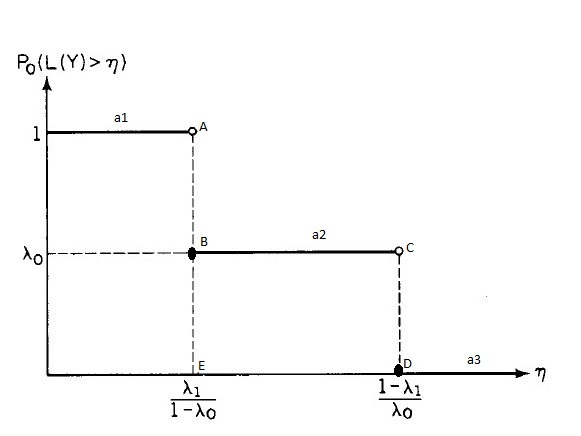
\includegraphics[scale=0.8]{img.jpg} 


\textbf{(fig-2 curve for threshold and randomization selection for a binary channel)}


Let $\eta_0$ be the smallest number such that
\begin{eqnarray}
&\mathbb{P}_0(p_1(Y) > \eta_0 p_0(Y)) \leq \alpha & 
\end{eqnarray}
$\eta_0 =\left\{ \begin{tabular}{c c c }
$\frac{1-\lambda_1}{\lambda_0}$ & $\alpha \in [0,\lambda_0)$ & $(as \,\eta_0 \,should\,\, satisfy \, equation (5),\,see\, the\, part\, a_3\, in\, above\, fig-2)$\\
\\
$\frac{\lambda_1}{1-\lambda_0}$ & $\alpha \in [\lambda_0,1)$ & $(see\,\,the\,\,part\,\,a_2\,\,in\,\,above\,\,figure-2) $ \\
\\
arbitrary & $ \alpha = 1$

\end{tabular}\right.$ \\

If $\mathbb{P}_0(p_1(Y) > \eta_0 p_0(Y)) <\alpha$ ,choose  $$\gamma_0 = \frac{\alpha-\mathbb{P}_0(p_1(Y) > \eta_0 p_0(Y))}{\mathbb{P}_0(p_1(Y) = \eta_0 p_0(Y))}$$ \\
If $\alpha \in [0,\lambda_0)$ \\
$\gamma_0 = \frac{\alpha-0}{\mathbb{P}_0(p_1(Y) = \eta_0 p_0(Y))}$ and \\

$\mathbb{P}_0(p_1(Y) = \eta_0 p_0(Y)) = \lambda_0-0$   \{Jumpsize at threshold, CD in fig-2\} \\

$\Rightarrow\gamma_0 = \frac{\alpha}{\lambda_0}$ \\

If $\alpha \in [\lambda_0,1)$\\ $\mathbb{P}_0(p_1(Y) = \eta_0 p_0(Y)) = 1-\lambda_0$ \{jumpsize at threshold, AB in fig-2\} \\

$\Rightarrow\gamma_0 = \frac{\alpha-\lambda_0}{1-\lambda_0}$ \\
$$\Rightarrow\gamma_0 =\left\{ \begin{tabular}{c c c }
$\frac{\alpha}{\lambda_0}$ & $\alpha \in [0,\lambda_0)$ \\
\\

$\frac{\alpha-\lambda_0}{1-\lambda_0}$ & $\alpha \in [\lambda_0,1)$ \\
\\
arbitrary & $ \alpha = 1$

\end{tabular}\right.$$ \\
If $\alpha \in [0,\lambda_0)$ 
$$\tilde{\delta}_{NP} (y) =\left\{ \begin{tabular}{c c}
$\frac{\alpha}{\lambda_0}$  & $ if y=1$ \\
\\

$0$  & $ if y=0$  \\
\end{tabular}\right.$$  \\
If $\alpha \in [\lambda_0,1]$
$$\tilde{\delta}_{NP} (y) =\left\{ \begin{tabular}{c c}
$1$  & $ if y=1$  \\
\\

$\frac{\alpha - \lambda_0}{1-\lambda_0}$  & $ if y=0$ \\

\end{tabular}\right.$$  \\

The detection probability of the Neyman-Pearson test is given by $\mathbb{P}_D (\tilde{\delta}_{NP}) =\mathbb{P}_1(L(Y) > \eta_0) + \gamma_0 \mathbb{P}_1(L(Y) = \eta_0)$ ,

$$\mathbb{P}_D (\tilde{\delta}_{NP}) =\left\{ \begin{tabular}{c c}
$\frac{\alpha (1-\lambda_1)}{\lambda_0}$ & $\alpha \in [0,\lambda_0)$ \\
\\

$(1-\lambda_1) + \frac{\lambda_1 (\alpha -\lambda_0)}{1-\lambda_0}$ & $\alpha \in [\lambda_0,1]$

\end{tabular} \right.$$ \\


\section{Composite Hypothesis Test}
The hypothesis testing problems discussed in the previous lectures are sometimes known as simple hypothesis testing problems because each of the two hypotheses corresponds to only a single distribution for the observation.In many hypothesis testing problems,however,there are many possible distributions that can occur under each of the hypotheses.Hypotheses of this type are known as \textit{Composite Hypotheses}.\\


To model the most general type of composite-hypotheses testing problem,we can consider a family of probability distributions on $\Gamma$ indexed by a parameter $\theta$ taking values in a parameter set $\Lambda$.That is we have a family: \\
$$\{P_\theta;\theta \in \Lambda\}$$

$\Lambda$=\{set of all possible states of nature\}\\

Example:\\
For the simple hypothesis test $\Lambda$ =\{0,1\}.More generally,we might have a parameter space that is the union of two disjoint parameter sets $\Lambda_0$ and $\Lambda_1$ representing the ranges of the parameter under the two hypothesis. \\  \\
\textbf{Bayesian Formulation:}

In a Bayesian formulation of the composite hypothesis testing problem,we assume that the parameter is a random quantity,$\Theta$,taking on the values in $\Lambda$.
i.e\\
$$\Theta : \Omega \to \Lambda $$   
In this case $ P_\theta$ is interpreted as the conditional distribution of Y given that $\Theta = \theta$.\\
$$ P_\theta \{ Y = y \} = \mathbb{P} \{ Y=y | \Theta = \theta\} $$ \\
we will consider only non randomized decision rules,$$ \Theta \in \Lambda_0  or  \Lambda_1$$ \\
To choose an optimum decision rule,assign cost to our decisions through a cost function $ C_i (\theta)$ where \\
$ C_i (\theta)$ = cost of choosing decision $i \in \{0,1\}$ when $Y \sim P_\theta$.

Assume that C is nonnegative and bounded.
For a decision rule $\delta$ Conditional Risk is
\begin{eqnarray}
& R_\theta (\delta) = \mathbb{E} [ C_{ \delta_y } (\theta)]&  
 \end{eqnarray} \\
where $\mathbb{E}$ denotes expectation assuming that $ Y \sim P_\theta$.Bayes risk  can be defined as $$ r(\delta) = \mathbb{E} [ R_\Theta (\delta)] $$\\

Bayes rule defined as minimization of $r(\delta)$.

$$ r(\delta) = \mathbb{E} [ R_\Theta (\delta)]\,\,\,\,\,\, \{using\,\, equation(6)\} $$ 

 $$ = \mathbb{E}[\mathbb{E}[ C_{ \delta_y } (\Theta)]]$$
$$ = \mathbb{E}[\mathbb{E}[ C_{ \delta_y } (\theta) | \Theta ]] $$
$$ = \mathbb{E}[\mathbb{E}[ C_{ \delta_y } (\Theta) | Y=y ]] \forall \{ y \in \Lambda \}$$

Minimizing $r(\delta)$ is same as minimizing $\mathbb{E}[\mathbb{E}[ C_{ \delta_y } (\Theta) | Y=y ]$. \\
Since $\delta_y $ can only be 0 or 1 ,we thus see that Bayes rule is given by,
$$\delta_y = argmin_{i \in \{0,1\}} \mathbb{E}[C_{ \delta_y } (\Theta) | Y=y]$$ \\
We choose $\delta (y)$ to be the decision that minimizes the posterior cost.
\begin{large}


$\delta_y$ =$\mathbb{I}_{\{\mathbb{E}[C_1(\Theta) | Y=y] < \mathbb{E}[C_0(\Theta) | Y=y]\}}$
\end{large} \\

$\delta (y)$ chooses the hypothesis that is least costly.For example- when $\Lambda =\{0,1\}$ ,$\delta (y)$ reduces with the Bayes rule for simple hypothesis test. \\

Assume costs being uniform i.e $ C_i (\theta) = C_{ij}$        ,  $\forall$    $ \theta \in \Lambda_j $.\\
=$ \int_{\theta \in \Lambda_1} C_{11} d\mathbb{P}_{(\theta | Y=y)}$ + $ \int_{\theta \in \Lambda_0} C_{10} d\mathbb{P}_{(\theta | Y=y)}$ \\

=$ C_{11} \mathbb{P}(\Theta \in \Lambda_1  | Y=y)$  + $C_{10}  \mathbb{P}(\Theta \in \Lambda_0  | Y=y)$ 


$< C_{01} \mathbb{P}(\Theta \in \Lambda_1  | Y=y)$  +$C_{00}  \mathbb{P}(\Theta \in \Lambda_0  | Y=y)$   $\{$ under the assumption $ C_{11} < C_{01}  \}$ \\
We can also write \\
$$\Gamma_1 =\left\{ \frac{C_{10}-C_{00}}{C_{01}-C_{11}} < \frac{\mathbb{P}(\Theta \in \Lambda_1  | Y=y)}{\mathbb{P}(\Theta \in \Lambda_0  | Y=y)} \right\}$$ 

where $\mathbb{P}(\Theta \in \Lambda_j  | Y=y)$ denotes the conditional probability that $\Theta$ lies in $\Lambda_j$ given that $Y=y$.Assume Y has conditional densities $\mathbb{P} (y | \Theta \in \Lambda_j)$ for j=0,1. \\
Bayes formula implies that : $$\mathbb{P} ( \Theta \in \Lambda_j | Y=y) = \frac{{\mathbb{P} (Y=y | \Theta \in \Lambda_j)}{\mathbb{P}(\Theta \in \Lambda_j)}}{\mathbb{P}(y)} , j=0,1$$ \\
We can write $\Gamma_1$ as $$\Gamma_1 =\left\{ \frac{{d\mathbb{P} (Y=y | \Theta \in \Lambda_1)}{\mathbb{P}(\Theta \in \Lambda_1)}}{{d\mathbb{P} (Y=y | \Theta \in \Lambda_0)}{\mathbb{P}(\Theta \in \Lambda_0)}} > \frac{C_{10}-C_{00}}{C_{01}-C_{11}}\right\}$$
For general case ,Let $\Theta \sim W, Y\sim \mathbb{P}_\theta ,\theta \in \Lambda $ \\
$$d\mathbb{P}[Y\leq y | \Theta \in \Lambda_j] = \int_\Lambda {\mathbb{P}_\theta(y) dW_j(\theta)},where$$

$$ dW_j(\theta) =\left\{ \begin{tabular}{c c} 
$0$ & $\theta \notin \Lambda_j$\\
$\frac{dW(\theta)}{\mathbb{P}\{\theta \in \Lambda_j\}}$ & $\theta \in \Lambda_j$

\end{tabular}\right. $$ 

\end{document}